%&latexf
\documentclass[]{kclthesis}

%===========================================================
% Change below accordingly and remove``\red{}''
%===========================================================

% TODO: WILL NEED TO MAKE THIS INTO A TABLE TO ALIGN IT PROPERLY

\department{Informatics} %use the right department
\modulecode{7CCSMPRJ} %Use the right module code
\submissiontitle{Individual Project Submission 2024 - 2025}
\author{Siddharth Kishor Samarth}
\studentnumber{K24012370}
\programme{MSc. Advanced Computing}
\title{GluCORRECT - Harnessing Artificial Intelligence to scrutinize Hypoglycemia in hospitalised patients with diabetes to classify, anticipate and analyse hypoglycemic episodes [Knowledge Exchange Project with NHS England]}
\supervisor{Dr. Rita Borgo}
\wordcount{\red{==== Word count goes here ====}}


\ReleaseProject{1} %Replace 0 by 1 if release project; Replace 0 by 2 if not release project

%===========================================================


% nomenclature 
\usepackage[intoc]{nomencl} 
%\makenomenclature
\makeindex
% glossaries
\usepackage[toc, acronym]{glossaries} 
\usepackage{float}
\usepackage{array} % for table content col / row alignment
\usepackage{hyperref}
\usepackage[utf8]{inputenc}
\usepackage{graphbox}
\usepackage{hyperref}

\usepackage{soul} % highlighting text

\linespread{1}
\newfam\msbfam
\def\Bbb#1{\fam\msbfam\relax#1}

\newtheorem{theorem}{Theorem}[section]
\newtheorem{exa}{Example}[section]
\newtheorem{corollary}[theorem]{Corollary}
\newtheorem{lemma}[theorem]{Lemma}
\newtheorem{proposition}[theorem]{Proposition}

\theoremstyle{definition}
\newtheorem{definition}[theorem]{Definition}
\newtheorem{remark}[theorem]{Remark}
\newtheorem{notation}[theorem]{Notation}
\newtheorem{assumption}[theorem]{Assumption}
\newtheorem{conjecture}[theorem]{Conjecture}

\newcommand{\ind}{1\hspace{-2.1mm}{1}} %Indicator Function
\newcommand{\I}{\mathtt{i}}
\newcommand{\D}{\mathrm{d}}
\newcommand{\E}{\mathrm{e}}
\newcommand{\RR}{\mathbb{R}}
\newcommand{\sgn}{\mathrm{sgn}}
\newcommand{\atanh}{\mathrm{arctanh}}
\def\equalDistrib{\,{\buildrel \Delta \over =}\,}
\numberwithin{equation}{section}
\def\blue#1{\textcolor{blue}{#1}}
\def\red#1{\textcolor{red}{#1}}

\setcounter{tocdepth}{5}
\setcounter{secnumdepth}{5}

% customize your general setup here
%\title{\red{Project title goes here}}
%\author{\red{Your name goes here}}


\begin{document}
\pagenumbering{gobble}


%%%%%% depends what you like, might try out the other frontpage as well
\maketitle 		% official styled layout
\maketitleTwo 	% adapted layout which looks nicer from my point of view.

%%%%%% empty page after main page.
\newpage
\thispagestyle{empty}
\mbox{}
\newpage
%%%%%% Acknowledgements, Abstract, Nomenclature
% \section{Template Descriptions}

\subsection{Template Folder Structure}
	After unzip the Latex template, you will find the following folders:
\begin{itemize}
	\item \textbf{``root'' folder:} The file ``thesis.tex'' is the master file of the whole document, which defines the structure of the chapters and other settings.
	\item \textbf{``contents'' folder:}  This is the folder for all chapters. Use the path \begin{verbatim}contents/chapter_filename\end{verbatim} when including chapters. The following files can be found in this folder.
	\begin{itemize}
		\item acknowledgements.tex: the contents of the Acknowledgement chapter. 
		\item abstract.tex: the contents of the Abstract chapter. 
		\item nomenclature.tex: the contents of the Nomenclature chapter. 
		\item introduction.tex: the contents of the Introduction chapter. 
		\item background.tex: the contents of the Background Theories chapter. 
		\item main.tex: the contents of the chapter regarding the main results. 
		\item conclusion.tex: the contents of the Conclusion chapter. 
		\item app\_1.tex: the contents of the Appendix chapter. 
		\item sample\_1.bib: the bibtex file for references. Remember to run ``bibtex'' to update the list of reference section.
		\item TemplateDescriptions.tex: this is the content of this chapter (Template Description). Remove the line \begin{verbatim} \section{Template Descriptions}

\subsection{Template Folder Structure}
	After unzip the Latex template, you will find the following folders:
\begin{itemize}
	\item \textbf{``root'' folder:} The file ``thesis.tex'' is the master file of the whole document, which defines the structure of the chapters and other settings.
	\item \textbf{``contents'' folder:}  This is the folder for all chapters. Use the path \begin{verbatim}contents/chapter_filename\end{verbatim} when including chapters. The following files can be found in this folder.
	\begin{itemize}
		\item acknowledgements.tex: the contents of the Acknowledgement chapter. 
		\item abstract.tex: the contents of the Abstract chapter. 
		\item nomenclature.tex: the contents of the Nomenclature chapter. 
		\item introduction.tex: the contents of the Introduction chapter. 
		\item background.tex: the contents of the Background Theories chapter. 
		\item main.tex: the contents of the chapter regarding the main results. 
		\item conclusion.tex: the contents of the Conclusion chapter. 
		\item app\_1.tex: the contents of the Appendix chapter. 
		\item sample\_1.bib: the bibtex file for references. Remember to run ``bibtex'' to update the list of reference section.
		\item TemplateDescriptions.tex: this is the content of this chapter (Template Description). Remove the line \begin{verbatim} \section{Template Descriptions}

\subsection{Template Folder Structure}
	After unzip the Latex template, you will find the following folders:
\begin{itemize}
	\item \textbf{``root'' folder:} The file ``thesis.tex'' is the master file of the whole document, which defines the structure of the chapters and other settings.
	\item \textbf{``contents'' folder:}  This is the folder for all chapters. Use the path \begin{verbatim}contents/chapter_filename\end{verbatim} when including chapters. The following files can be found in this folder.
	\begin{itemize}
		\item acknowledgements.tex: the contents of the Acknowledgement chapter. 
		\item abstract.tex: the contents of the Abstract chapter. 
		\item nomenclature.tex: the contents of the Nomenclature chapter. 
		\item introduction.tex: the contents of the Introduction chapter. 
		\item background.tex: the contents of the Background Theories chapter. 
		\item main.tex: the contents of the chapter regarding the main results. 
		\item conclusion.tex: the contents of the Conclusion chapter. 
		\item app\_1.tex: the contents of the Appendix chapter. 
		\item sample\_1.bib: the bibtex file for references. Remember to run ``bibtex'' to update the list of reference section.
		\item TemplateDescriptions.tex: this is the content of this chapter (Template Description). Remove the line \begin{verbatim} \include{contents/TemplateDescriptions}\end{verbatim} from ``thesis.tex'' which will remove the Chapter ``Template Descriptions'' from the document.
	\end{itemize}
	Create a new chapter file if necessary.
	\item \textbf{``figures'' folder:} This is the folder for all figures. Use the path \begin{verbatim}contents/figure_filename\end{verbatim} when including figures.
\end{itemize}

contents/sample1
bibtex, run bibtex

\subsection{Student and Project Information}
	The master file of this template is ``thesis.tex''. Change the following lines accordingly in ``thesis.tex'' to include your information.

\begin{verbatim}
%===========================================================
% Change below accordingly and remove``\red{}''
%===========================================================
\modulecode{\red{7CCSMPRJ/7CCSMUIP}} %Use the right module code
\submissiontitle{Individual Project Submission \red{20XX/XX (Replace XX by year)}}
\studentnumber{\red{Student number goes here}}
\programme{\red{Programme title goes here}}
\supervisor{\red{Supervisor's name goes here}}
\wordcount{\red{Word count goes here}}
\title{\red{Project title goes here}}
\author{\red{Your name goes here}}
\ReleaseProject{0} %Replace 0 by 1 if release project; Replace 0 by 2 if not release project
\department{\red{Engineering/Information}} %use the right department
%===========================================================
\end{verbatim}

	Remove the line \begin{verbatim} \include{contents/TemplateDescriptions}\end{verbatim} from ``thesis.tex'' which will remove the Chapter ``Template Descriptions'' from the document.\\
	
	Replace the image ``signature.png'' in the folder ``figures'' by your signature image in ``png'' format.\end{verbatim} from ``thesis.tex'' which will remove the Chapter ``Template Descriptions'' from the document.
	\end{itemize}
	Create a new chapter file if necessary.
	\item \textbf{``figures'' folder:} This is the folder for all figures. Use the path \begin{verbatim}contents/figure_filename\end{verbatim} when including figures.
\end{itemize}

contents/sample1
bibtex, run bibtex

\subsection{Student and Project Information}
	The master file of this template is ``thesis.tex''. Change the following lines accordingly in ``thesis.tex'' to include your information.

\begin{verbatim}
%===========================================================
% Change below accordingly and remove``\red{}''
%===========================================================
\modulecode{\red{7CCSMPRJ/7CCSMUIP}} %Use the right module code
\submissiontitle{Individual Project Submission \red{20XX/XX (Replace XX by year)}}
\studentnumber{\red{Student number goes here}}
\programme{\red{Programme title goes here}}
\supervisor{\red{Supervisor's name goes here}}
\wordcount{\red{Word count goes here}}
\title{\red{Project title goes here}}
\author{\red{Your name goes here}}
\ReleaseProject{0} %Replace 0 by 1 if release project; Replace 0 by 2 if not release project
\department{\red{Engineering/Information}} %use the right department
%===========================================================
\end{verbatim}

	Remove the line \begin{verbatim} \section{Template Descriptions}

\subsection{Template Folder Structure}
	After unzip the Latex template, you will find the following folders:
\begin{itemize}
	\item \textbf{``root'' folder:} The file ``thesis.tex'' is the master file of the whole document, which defines the structure of the chapters and other settings.
	\item \textbf{``contents'' folder:}  This is the folder for all chapters. Use the path \begin{verbatim}contents/chapter_filename\end{verbatim} when including chapters. The following files can be found in this folder.
	\begin{itemize}
		\item acknowledgements.tex: the contents of the Acknowledgement chapter. 
		\item abstract.tex: the contents of the Abstract chapter. 
		\item nomenclature.tex: the contents of the Nomenclature chapter. 
		\item introduction.tex: the contents of the Introduction chapter. 
		\item background.tex: the contents of the Background Theories chapter. 
		\item main.tex: the contents of the chapter regarding the main results. 
		\item conclusion.tex: the contents of the Conclusion chapter. 
		\item app\_1.tex: the contents of the Appendix chapter. 
		\item sample\_1.bib: the bibtex file for references. Remember to run ``bibtex'' to update the list of reference section.
		\item TemplateDescriptions.tex: this is the content of this chapter (Template Description). Remove the line \begin{verbatim} \include{contents/TemplateDescriptions}\end{verbatim} from ``thesis.tex'' which will remove the Chapter ``Template Descriptions'' from the document.
	\end{itemize}
	Create a new chapter file if necessary.
	\item \textbf{``figures'' folder:} This is the folder for all figures. Use the path \begin{verbatim}contents/figure_filename\end{verbatim} when including figures.
\end{itemize}

contents/sample1
bibtex, run bibtex

\subsection{Student and Project Information}
	The master file of this template is ``thesis.tex''. Change the following lines accordingly in ``thesis.tex'' to include your information.

\begin{verbatim}
%===========================================================
% Change below accordingly and remove``\red{}''
%===========================================================
\modulecode{\red{7CCSMPRJ/7CCSMUIP}} %Use the right module code
\submissiontitle{Individual Project Submission \red{20XX/XX (Replace XX by year)}}
\studentnumber{\red{Student number goes here}}
\programme{\red{Programme title goes here}}
\supervisor{\red{Supervisor's name goes here}}
\wordcount{\red{Word count goes here}}
\title{\red{Project title goes here}}
\author{\red{Your name goes here}}
\ReleaseProject{0} %Replace 0 by 1 if release project; Replace 0 by 2 if not release project
\department{\red{Engineering/Information}} %use the right department
%===========================================================
\end{verbatim}

	Remove the line \begin{verbatim} \include{contents/TemplateDescriptions}\end{verbatim} from ``thesis.tex'' which will remove the Chapter ``Template Descriptions'' from the document.\\
	
	Replace the image ``signature.png'' in the folder ``figures'' by your signature image in ``png'' format.\end{verbatim} from ``thesis.tex'' which will remove the Chapter ``Template Descriptions'' from the document.\\
	
	Replace the image ``signature.png'' in the folder ``figures'' by your signature image in ``png'' format.\end{verbatim} from ``thesis.tex'' which will remove the Chapter ``Template Descriptions'' from the document.
	\end{itemize}
	Create a new chapter file if necessary.
	\item \textbf{``figures'' folder:} This is the folder for all figures. Use the path \begin{verbatim}contents/figure_filename\end{verbatim} when including figures.
\end{itemize}

contents/sample1
bibtex, run bibtex

\subsection{Student and Project Information}
	The master file of this template is ``thesis.tex''. Change the following lines accordingly in ``thesis.tex'' to include your information.

\begin{verbatim}
%===========================================================
% Change below accordingly and remove``\red{}''
%===========================================================
\modulecode{\red{7CCSMPRJ/7CCSMUIP}} %Use the right module code
\submissiontitle{Individual Project Submission \red{20XX/XX (Replace XX by year)}}
\studentnumber{\red{Student number goes here}}
\programme{\red{Programme title goes here}}
\supervisor{\red{Supervisor's name goes here}}
\wordcount{\red{Word count goes here}}
\title{\red{Project title goes here}}
\author{\red{Your name goes here}}
\ReleaseProject{0} %Replace 0 by 1 if release project; Replace 0 by 2 if not release project
\department{\red{Engineering/Information}} %use the right department
%===========================================================
\end{verbatim}

	Remove the line \begin{verbatim} \section{Template Descriptions}

\subsection{Template Folder Structure}
	After unzip the Latex template, you will find the following folders:
\begin{itemize}
	\item \textbf{``root'' folder:} The file ``thesis.tex'' is the master file of the whole document, which defines the structure of the chapters and other settings.
	\item \textbf{``contents'' folder:}  This is the folder for all chapters. Use the path \begin{verbatim}contents/chapter_filename\end{verbatim} when including chapters. The following files can be found in this folder.
	\begin{itemize}
		\item acknowledgements.tex: the contents of the Acknowledgement chapter. 
		\item abstract.tex: the contents of the Abstract chapter. 
		\item nomenclature.tex: the contents of the Nomenclature chapter. 
		\item introduction.tex: the contents of the Introduction chapter. 
		\item background.tex: the contents of the Background Theories chapter. 
		\item main.tex: the contents of the chapter regarding the main results. 
		\item conclusion.tex: the contents of the Conclusion chapter. 
		\item app\_1.tex: the contents of the Appendix chapter. 
		\item sample\_1.bib: the bibtex file for references. Remember to run ``bibtex'' to update the list of reference section.
		\item TemplateDescriptions.tex: this is the content of this chapter (Template Description). Remove the line \begin{verbatim} \section{Template Descriptions}

\subsection{Template Folder Structure}
	After unzip the Latex template, you will find the following folders:
\begin{itemize}
	\item \textbf{``root'' folder:} The file ``thesis.tex'' is the master file of the whole document, which defines the structure of the chapters and other settings.
	\item \textbf{``contents'' folder:}  This is the folder for all chapters. Use the path \begin{verbatim}contents/chapter_filename\end{verbatim} when including chapters. The following files can be found in this folder.
	\begin{itemize}
		\item acknowledgements.tex: the contents of the Acknowledgement chapter. 
		\item abstract.tex: the contents of the Abstract chapter. 
		\item nomenclature.tex: the contents of the Nomenclature chapter. 
		\item introduction.tex: the contents of the Introduction chapter. 
		\item background.tex: the contents of the Background Theories chapter. 
		\item main.tex: the contents of the chapter regarding the main results. 
		\item conclusion.tex: the contents of the Conclusion chapter. 
		\item app\_1.tex: the contents of the Appendix chapter. 
		\item sample\_1.bib: the bibtex file for references. Remember to run ``bibtex'' to update the list of reference section.
		\item TemplateDescriptions.tex: this is the content of this chapter (Template Description). Remove the line \begin{verbatim} \include{contents/TemplateDescriptions}\end{verbatim} from ``thesis.tex'' which will remove the Chapter ``Template Descriptions'' from the document.
	\end{itemize}
	Create a new chapter file if necessary.
	\item \textbf{``figures'' folder:} This is the folder for all figures. Use the path \begin{verbatim}contents/figure_filename\end{verbatim} when including figures.
\end{itemize}

contents/sample1
bibtex, run bibtex

\subsection{Student and Project Information}
	The master file of this template is ``thesis.tex''. Change the following lines accordingly in ``thesis.tex'' to include your information.

\begin{verbatim}
%===========================================================
% Change below accordingly and remove``\red{}''
%===========================================================
\modulecode{\red{7CCSMPRJ/7CCSMUIP}} %Use the right module code
\submissiontitle{Individual Project Submission \red{20XX/XX (Replace XX by year)}}
\studentnumber{\red{Student number goes here}}
\programme{\red{Programme title goes here}}
\supervisor{\red{Supervisor's name goes here}}
\wordcount{\red{Word count goes here}}
\title{\red{Project title goes here}}
\author{\red{Your name goes here}}
\ReleaseProject{0} %Replace 0 by 1 if release project; Replace 0 by 2 if not release project
\department{\red{Engineering/Information}} %use the right department
%===========================================================
\end{verbatim}

	Remove the line \begin{verbatim} \include{contents/TemplateDescriptions}\end{verbatim} from ``thesis.tex'' which will remove the Chapter ``Template Descriptions'' from the document.\\
	
	Replace the image ``signature.png'' in the folder ``figures'' by your signature image in ``png'' format.\end{verbatim} from ``thesis.tex'' which will remove the Chapter ``Template Descriptions'' from the document.
	\end{itemize}
	Create a new chapter file if necessary.
	\item \textbf{``figures'' folder:} This is the folder for all figures. Use the path \begin{verbatim}contents/figure_filename\end{verbatim} when including figures.
\end{itemize}

contents/sample1
bibtex, run bibtex

\subsection{Student and Project Information}
	The master file of this template is ``thesis.tex''. Change the following lines accordingly in ``thesis.tex'' to include your information.

\begin{verbatim}
%===========================================================
% Change below accordingly and remove``\red{}''
%===========================================================
\modulecode{\red{7CCSMPRJ/7CCSMUIP}} %Use the right module code
\submissiontitle{Individual Project Submission \red{20XX/XX (Replace XX by year)}}
\studentnumber{\red{Student number goes here}}
\programme{\red{Programme title goes here}}
\supervisor{\red{Supervisor's name goes here}}
\wordcount{\red{Word count goes here}}
\title{\red{Project title goes here}}
\author{\red{Your name goes here}}
\ReleaseProject{0} %Replace 0 by 1 if release project; Replace 0 by 2 if not release project
\department{\red{Engineering/Information}} %use the right department
%===========================================================
\end{verbatim}

	Remove the line \begin{verbatim} \section{Template Descriptions}

\subsection{Template Folder Structure}
	After unzip the Latex template, you will find the following folders:
\begin{itemize}
	\item \textbf{``root'' folder:} The file ``thesis.tex'' is the master file of the whole document, which defines the structure of the chapters and other settings.
	\item \textbf{``contents'' folder:}  This is the folder for all chapters. Use the path \begin{verbatim}contents/chapter_filename\end{verbatim} when including chapters. The following files can be found in this folder.
	\begin{itemize}
		\item acknowledgements.tex: the contents of the Acknowledgement chapter. 
		\item abstract.tex: the contents of the Abstract chapter. 
		\item nomenclature.tex: the contents of the Nomenclature chapter. 
		\item introduction.tex: the contents of the Introduction chapter. 
		\item background.tex: the contents of the Background Theories chapter. 
		\item main.tex: the contents of the chapter regarding the main results. 
		\item conclusion.tex: the contents of the Conclusion chapter. 
		\item app\_1.tex: the contents of the Appendix chapter. 
		\item sample\_1.bib: the bibtex file for references. Remember to run ``bibtex'' to update the list of reference section.
		\item TemplateDescriptions.tex: this is the content of this chapter (Template Description). Remove the line \begin{verbatim} \include{contents/TemplateDescriptions}\end{verbatim} from ``thesis.tex'' which will remove the Chapter ``Template Descriptions'' from the document.
	\end{itemize}
	Create a new chapter file if necessary.
	\item \textbf{``figures'' folder:} This is the folder for all figures. Use the path \begin{verbatim}contents/figure_filename\end{verbatim} when including figures.
\end{itemize}

contents/sample1
bibtex, run bibtex

\subsection{Student and Project Information}
	The master file of this template is ``thesis.tex''. Change the following lines accordingly in ``thesis.tex'' to include your information.

\begin{verbatim}
%===========================================================
% Change below accordingly and remove``\red{}''
%===========================================================
\modulecode{\red{7CCSMPRJ/7CCSMUIP}} %Use the right module code
\submissiontitle{Individual Project Submission \red{20XX/XX (Replace XX by year)}}
\studentnumber{\red{Student number goes here}}
\programme{\red{Programme title goes here}}
\supervisor{\red{Supervisor's name goes here}}
\wordcount{\red{Word count goes here}}
\title{\red{Project title goes here}}
\author{\red{Your name goes here}}
\ReleaseProject{0} %Replace 0 by 1 if release project; Replace 0 by 2 if not release project
\department{\red{Engineering/Information}} %use the right department
%===========================================================
\end{verbatim}

	Remove the line \begin{verbatim} \include{contents/TemplateDescriptions}\end{verbatim} from ``thesis.tex'' which will remove the Chapter ``Template Descriptions'' from the document.\\
	
	Replace the image ``signature.png'' in the folder ``figures'' by your signature image in ``png'' format.\end{verbatim} from ``thesis.tex'' which will remove the Chapter ``Template Descriptions'' from the document.\\
	
	Replace the image ``signature.png'' in the folder ``figures'' by your signature image in ``png'' format.\end{verbatim} from ``thesis.tex'' which will remove the Chapter ``Template Descriptions'' from the document.\\
	
	Replace the image ``signature.png'' in the folder ``figures'' by your signature image in ``png'' format. %Remove this line after reading
% \red{The content of ``Acknowledgements'' is in ``{\textbackslash}contents{\textbackslash}acknowledgements.tex''}

\mbox{}\newline\vspace{10mm} \mbox{}\LARGE
%
{\bf Acknowledgements} \normalsize \vspace{5mm}

\par I would like to express my sincerest gratitude towards my project supervisor, Dr. Rita Borgo, for her invaluable advice and consistent 
direction throughout the course of this project. Her mentorship and ideas have been instrumental in shaping the development of this work, 
leading to its successful completion.

\par I am also deeply thankful \& appreciative of my industry advisor, Dr. Piya Sen Gupta, for providing the dataset that has served as the 
foundation of this work. Her contributions have significantly enhanced the practical relevance and quality of this project.

\par Ultimately I would like to thank my friends and my parents, especially my dad, without whose sacrifices I would not be where I am today.
JELLO WORLD THIS IS TEST OF LATEX IN VSCODE

\red{The content of ``Abstract'' is in ``{\textbackslash}contents{\textbackslash}abstract.tex''}

\section*{Abstract}

% \begin{flushleft}

    \textbf{\underline{Project Variant:}} \textbf{ Variant 4 - Develop a weighted score and design score to predict risk of a hypoglycaemic episode before it occurs.} 

    \vspace{10pt}
    \par{It is well known that hypoglycemia as well as hyperglycemia are common adverse events in patients who receive blood sugar control medication, and they are also one of the most frequently cited causes of hospital admissions in people with diabetes. National quality improvement programmes from the Healthcare Quality Improvement Partnership (HQIP) and reviews of ambulance call-out data have shown that \textbf{\textit{lack of awareness}} by both affected individuals and their attendants is associated with a dramatically increased rate of complications, amongst other factors. Guy's and St. Thomas' NHS Foundation Trust (hereonwards referred to as GSTT) has found, after departmental investigation, that hypoglycemic episodes (also called "hypos") have been occurring unusually often, and seek to take measures to resolve such problems in a preventive manner as opposed to a corrective one. This research project has been undertaken in close collaboration with GSTT, one of the largest NHS trusts in the UK and an indispensable element of London's healthcare system, with almost 24000 staff across 5 major hospitals, handling over 3 million patients a year and generating an annual turnover of over \pounds3 billion.}

    \vspace{10pt}
    \par{This analytical study serves as a foundation and proof-of-concept to aid GSTT in pre-emptively reducing hypoglycemia within hospitalised inpatients, by utilising statistics \& machine learning techniques. Through exploratory data analysis I draw out relevant conclusions about the dataset around patient age, ethnicity and 
    
    I go on to identify the significant factors responsible for hypoglycemia within the dataset provided by the industry advisor from GSTT through exploratory data analysis, while also . I explore how they can be utilized to devise a risk score, to classify patients based on their risk of hypoglycemia. 
    
    HbA1c values identified as risky - 56 or so 
    eGFR 
    ethnicity
    major is glucose value 
    
 In conclusion, exhibit my findings with potential ways of applying them in practise in hospitals.}

    \vspace{10pt}

    \par{}

% \end{flushleft}

% \begin{itemize}
% 	\item A brief introduction to the project objectives
% 	\item A brief description of the main work of the project
% 	\item A brief description of the contributions, major findings, results achieved and principal conclusion of the project
% \end{itemize}

 All abbreviations and symbols used in the report must be listed and defined in alphabetic order.

\section*{Nomenclature}

\begin{flushleft}
\begin{minipage}{1\textwidth}
    	\centering
        \def\arraystretch{1.25}%
    	\begin{tabular}{ll}
			GSTT  & Guy's and St Thomas' NHS Foundation Trust \\
			HQIP & Healthcare Quality Improvement Partnership \\
			NCAPOP & National Clincal Audit \& Patient Outcomes Programme \\
			NDA   & National Database Audit  \\
    		NDISA & National Diabetes Inpatient Safety Audit \\  
    		NHS & The publicly funded healthcare system of the United Kingdom, \\ 
            & the National Health Service. \\
      
                
    	\end{tabular}
\end{minipage}

\end{flushleft}

\noindent\rule{8cm}{0.4pt} \\ % temporary horizontal rule
$a$ \qquad The number of angels per unit area\\
$A$ \qquad The area of the needle point\\
$c$ \qquad Speed of light in a vacuum inertial frame\\
$h$ \qquad Planck constant\\
LMI	\qquad Linear Matrix Inequalities\\
$N$ \qquad The number of angels per needle point
%%%%%% Table of contents

\pagenumbering{roman}
\setcounter{tocdepth}{4}
\tableofcontents
\newpage
%%%%%%%%%%%%%%%%%%%%%%%%%%%%%%%%%%%%%%%%%%%%%%%%%%%%
\thispagestyle{empty}
 
\listoffigures
 
\listoftables
 
\newpage
\fancyhead{}
\fancyfoot{}
\pagestyle{fancy} 
%\fancyhead{\sffamily\small \thepage}
%\fancyhead{\sffamily\small \nouppercase{\rightmark}}
\fancyhead[RO,LE]{\sffamily\small \thepage}
\fancyhead[LO,RE]{\sffamily\small \nouppercase{\rightmark}}
\renewcommand{\headrulewidth}{0.4pt}
\renewcommand{\footrulewidth}{0.0pt}
%%%%%%%%%%%%%%%%%%%%%%%%%%%%%%%%%%%%%%%%%%%%%%%%%%%%

%%%%%% Main content
\pagenumbering{arabic}

%Insert if necessary if more chapters are needed by creating a new .tex file in the folder ``contents'' and use \include{filename} to include the new chapter.
%Modify the section headings if necessary
%Insert more sections if necessary
\section{Introduction}
% It provides the background and context of the work.

\begin{flushleft}
Hypoglycemia is a condition that occurs when the human body’s blood glucose (sugar) level drops below the normal healthy range of 4.0 to 6.0 mmol/L. For the purposes of this project, severe hypoglycemia has been defined as a blood glucose of 2.2 mmol/L or lower. With glucose being the body’s main source of energy, hypoglycemia is a concern as it can disturb brain and bodily functions.  \\ \vspace{5pt}

Hypoglycemia is common in diabetics, especially those taking insulin, but it can occur in non-diabetics as well. Symptoms are rapid and successive, including feeling dizzy or sweating, shaking, feeling tired or weak and disorientated, unable to find one's bearing. \\ \vspace{5pt}

What is especially significant though, besides quick to appear symptoms, is that hypoglycemic episodes are dreadfully anxiety provoking, with practically every patient's main concern being if people around them would have the proper awareness of the necessary measures to take to resolve an episode should one occur. Even though remedial action is relatively simple (to provide the patient with sugary foods / liquids or solutions to restore blood glucose), it can lead to loss of consciousness \& memory, seizures, cardiac arrhythmias and even death if not taken speedily.    \\ \vspace{5pt}

Across GSTT, there are 0.5 million point of care glucose tests (POCT) carried out annually. GSTT possesses blood glucose / ketone data over the course of 1 year (Apr 2022-2023) with additional linked data including demographics, dates of admission and discharge, 
measurements including weight, blood pressure, HbA1c, renal function \& POCT. There is another kind of record they use called an ‘inpatient record’, and it was identified that the inpatient record misses approximately 10\% of glucose data due to operator error, as compared to the POCT glucose feed which contains more data. We would like to resolve this, while also analysing the available data in order to assist GSTT in detecting blood sugar related conditions, making measureable improvements to diabetic healthcare. \\ \vspace{5pt}

As evidenced by the National Diabetes Inpatient Safety Audit (NDISA) \hl{[insert reference]}, it has been recognized that severe hypoglycemia (blood glucose levels  2.2mmol/l) and recurrent severe hypoglycemia have been occurring relatively frequently at Guy’s and St. Thomas Hospitals (here onwards referred to as GSTT). The NDISA forms part of the National Database Audit (NDA), and it maintains that “The prevalence of diabetes continues to increase. In England between 2017-18 and 2021-22 prevalence of type 1 diabetes went up from 248,240 to 270,935 and the prevalence of type 2 and other diabetes from 2,952,695 to 3,336,980”, as of 2022. 

\end{flushleft}

\subsection{Aims and Objectives} 
% The problems and project objectives should be stated comprehensively. The motivations of the project should be presented. The techniques and approaches used to deal with the problem should be stated with justifications, and the contributions and main results achieved should be stated clearly. The structure of the report can be described briefly at the end see \autoref{sub:background}.



\subsubsection{Dissertation Length}
	The dissertation should be less than 15000 words.
	
\paragraph{Dissertation Length 2} ~\newline
	Refer to KEATS for suggested structure
	
\noindent \subparagraph{More subsections}~\newline
	
	

\subsection{Background and Literature Survey} \label{sub:background}
 It gives an overall picture about the work with a clear review of the relevant literature.  The background of the project should be given.  What have been done to deal with the problem should be stated clearly.  The pros and cons of various existing algorithms and approaches should be stated as well.  Differences between your proposed method and the existing ones should be briefly described. It is important to make sure that the discussion is structured and coherent; the key issues are summarised; key and relevant references are used critically analysed and the literature is covered comprehensively.

The following links may help on literature review:
\begin{itemize}
	\item \textbf{IEEE Xplore digital library} (\hyperref[http://ieeexplore.ieee.org]{http://ieeexplore.ieee.org/}): a resource for accessing IEEE published scientific and technical publications (You must be with King's network to get access to the digital library)
	\item \textbf{ScienceDirect.com} (\textbf{ScienceDirect.com} \hyperref[http://scienceDirect.com]{http://scienceDirect.com}): an electronic database offering journal papers not published by IEEE (You must be with King's network to get access to the database)
\end{itemize}

\subsection{Insert More Sections if Necessary}
\red{The content of ``Background'' is in ``{\textbackslash}contents{\textbackslash}background.tex''}

\section{Background theories \& Literature Survey} 

\begin{flushleft}
Various kinds of different prediction models have already been devised and developed for predicting hypoglycemia. Yi Wu and others have systematically compared, and evaluated the applicability of models in clinical practice in a paper in Biological Research for Nursing[1] 
where it was found that the major predictors were age, HbA1c, history of hypoglycemia, and insulin use. Lin Yang, Zhiguang Zhou have carried out similar research in the Frontiers in Public Health journal[2] uncovering risk factors that could possibly lead to hypoglycemic 
events, after employing various data driven models based on ML techniques such as neural networks, autoregressive / ensemble learning and such. \\ \vspace{5pt}

In silico proof of concept studies like the one from Zecchin[3] have also been researched to investigate how continuous glucose monitoring short-term glucose prediction algorithms could be exploited to recognise the run up to hypoglycemic episodes, allowing the patient to 
take appropriate countermeasures to mitigate events. They found that there was a significant reduction in both the time spent in a hypoglycemic event as well as the number 
of hypoglycemic events. \\ \vspace{5pt}

As this is a Knowledge Exchange Project (KEP) with NHS England I have been provided a real world dataset from GSTT. Medical data is difficult to obtain, and it rarely fits a research objective without needing much modification. 

% In this project I first go on to perform exploratory data analysis to better understand how the data is structured, how it is sourced, and how it can be visualised to extract maximum information.

\end{flushleft}
\red{The content of ``Main results'' is in ``{\textbackslash}contents{\textbackslash}introduction.tex''}

The chapter reports the contributions of your work.  For example, it could contain the following sub-sections to summarise the contribution of the project such as Theoretical Development, Analysis and Design, Implementation and Experimental Work, Results, Observation and Discussion.

\section{Objectives, Specification and Design}

	It recalls the objectives in a more detailed way to justify the development of a set of requirements and specifications, and identify a coherent set of issues to be addressed. It explains in detail the design and how the design can achieve the project aim (solve the problem).

\section{Methodology and Implementation}

	It presents and justifies the methodology used to deal with the problem and describes in detail the implementation procedures. The background theory presented in the previous chapter can be recalled to support the proposed implementation. The originality, novelty and contribution are to be demonstrated with the discussion of the strengths and limitations.

\section{Results, Analysis and Evaluation}
	It summarises the results obtained from the proposed design and methodology. The way to obtain the results should be described in detail. Analysis and evaluation have to be performed. Comparisons should be made. It should justifies if the project aims, objectives, requirements and specifications have been achieved.

\section{Legal, Social, Ethical and Professional Issues}
	A chapter gives a reasoned discussion about legal, social ethical and professional issues within the context of your project problem. You should also demonstrate that you are aware of the Code of Conduct \& Code of Good Practice issued by the British Computer Society (BSC) (\url{https://www.bcs.org/membership/become-a-member/bcs-code-of-conduct/}) for computer science project and Rule of Conduct issued by The Institution of Engineering and Technology (IET) (\url{https://www.theiet.org/about/governance/rules-of-conduct/}) for engineering project.  You should have applied their principles, where appropriate, as you carried out your project. You could consider aspects like: the effects of your project on the public well-being, security, software trustworthiness and risks, Intellectual Property and related issues, etc.


\section{Others}
\textcolor{red}{This section is for demonstration of equations, figures, tables, which is not required for the report.}
\subsection{Maths}
\begin{equation}\label{eq:BS}
\frac{\D S_t}{S_t} = r \D t + \sigma \D W_t,
\qquad S_0>0,
\end{equation}

The equation $\sigma = m a$ follows easily~\cite{Doe11}.


\subsection{Glossary and acronyms}

\newglossaryentry{Linux}
{
    name=latexlinux,
    description={Is a markup language specially suited for 
scientific documents}
}

\newglossaryentry{lvm}
{
    name=lvmformula,
    description={A mathematical expression}
}

\Glspl{Linux} and other Unix operating systems are better then Windows because they support \gls{lvm} out of the box~\cite{Joh11}\insertref{A ref is missing here}. 

\subsection{Figures}
Here is an example~\cite{JohSil05} of how to insert a picture:

\begin{figure}[!ht]
\centering
\subfigure{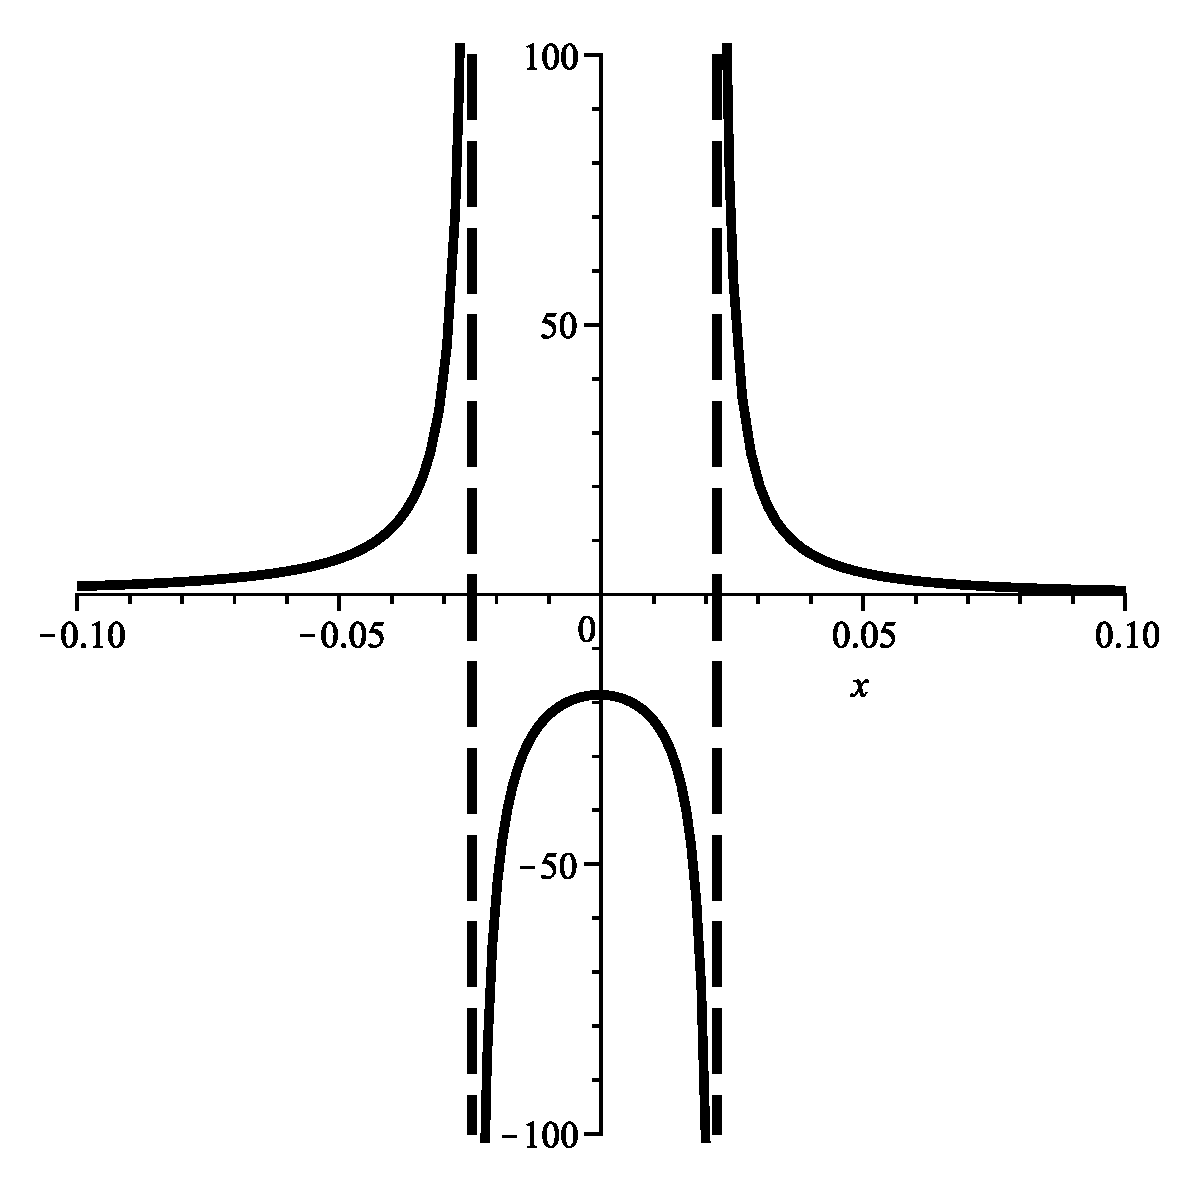
\includegraphics[scale=0.2]{figures/Picture.eps}}
\caption{This is the caption for the figure.}
\label{fig:Pict}
\end{figure}


\begin{figure}[!ht]
\centering
\missingfigure{If you know there will be a figure, but you still need to create it.}
\caption{This is the caption for the figure which is not even present.}
\label{fig:PictMis}
\end{figure}


Lorem ipsum dolor sit amet, consetetur sadipscing elitr, sed diam nonumy eirmod tempor invidunt ut labore et dolore magna aliquyam erat, sed diam voluptua. At vero eos et accusam et justo duo dolores et ea rebum. Stet clita kasd gubergren, no sea takimata sanctus est Lorem ipsum dolor sit amet. Lorem ipsum dolor sit amet, consetetur sadipscing elitr, sed diam nonumy eirmod tempor invidunt ut labore et dolore magna aliquyam erat, sed diam voluptua. At vero eos et accusam et justo duo dolores et ea rebum. Stet clita kasd gubergren, no sea takimata sanctus est Lorem ipsum dolor sit amet.\todo{This is a small Todo, please take care!}

or two side-by-side pictures:

\begin{figure}[!ht]
\centering
\subfigure{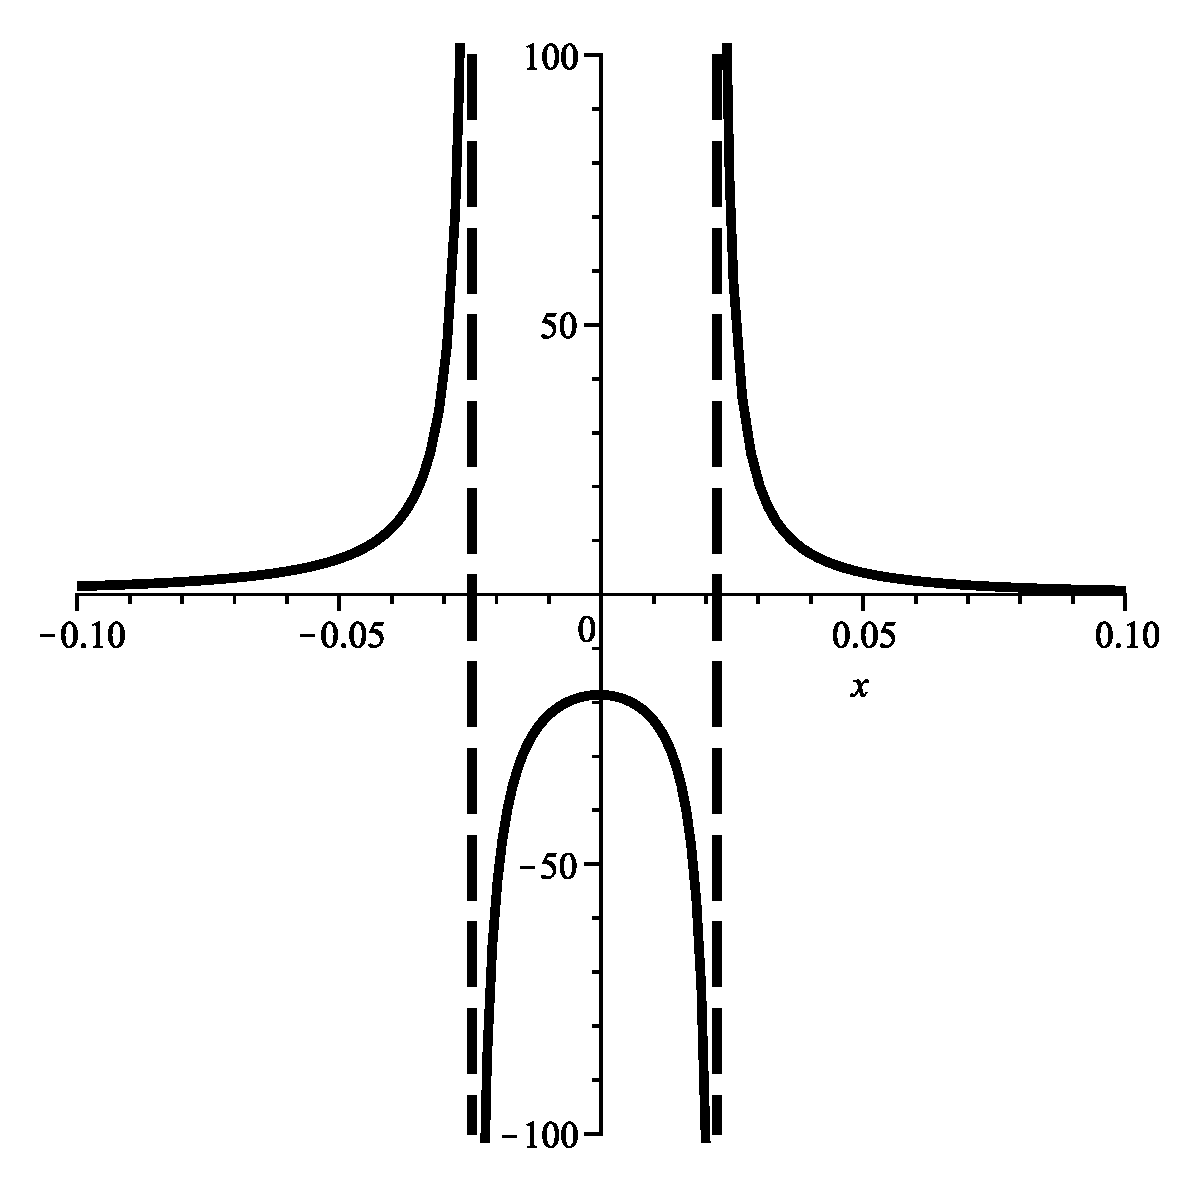
\includegraphics[scale=0.3]{figures/Picture.eps}}
\hspace{15pt}
\subfigure{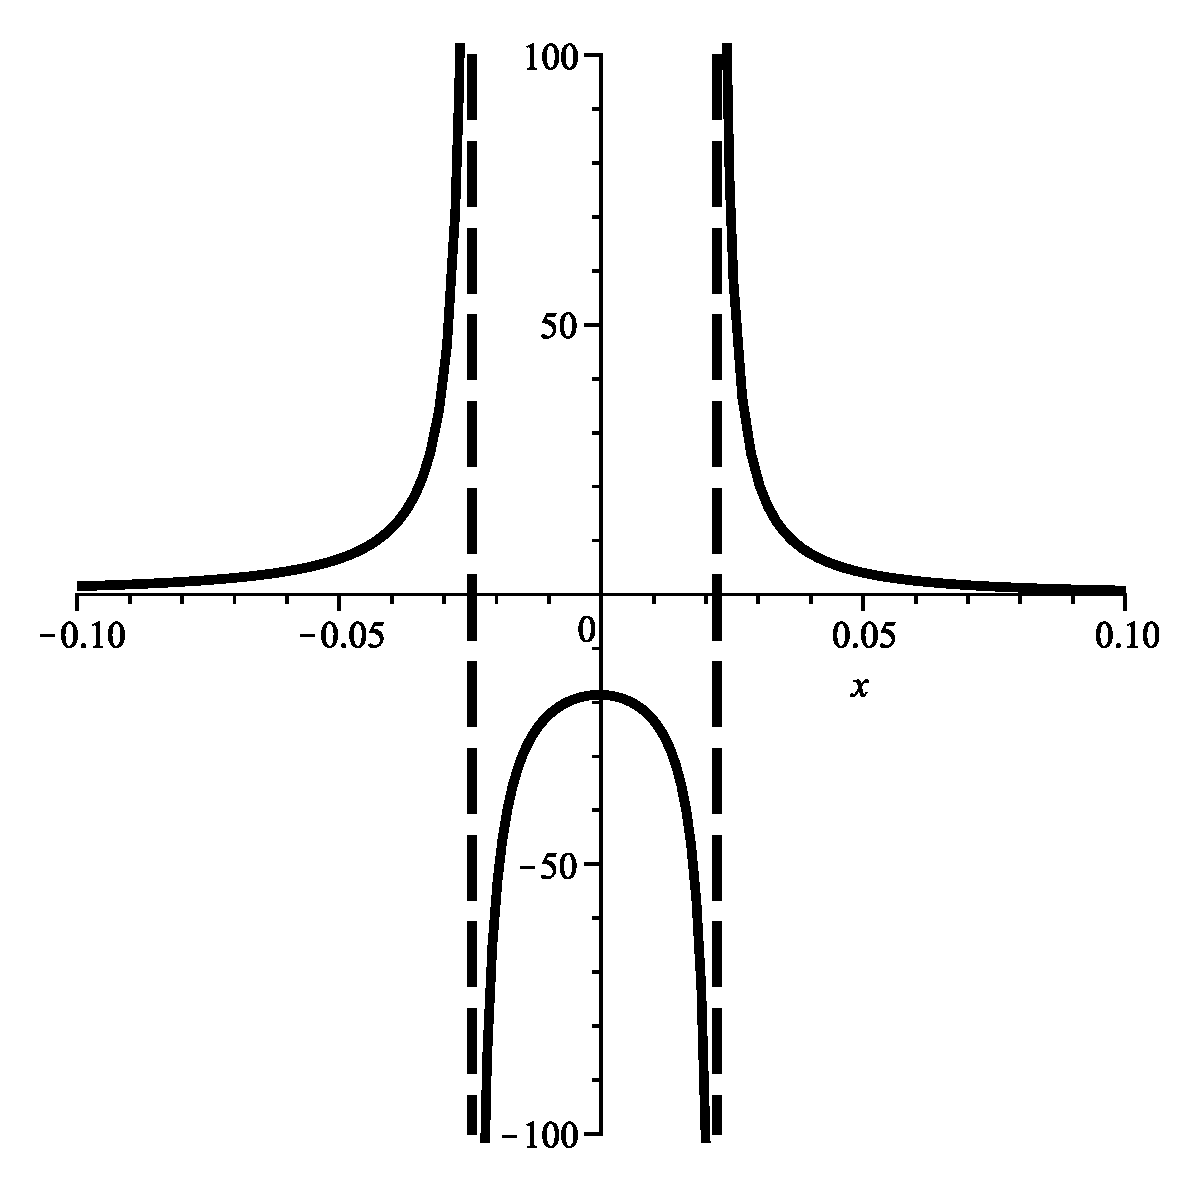
\includegraphics[scale=0.3]{figures/Picture.eps}}

\caption{Another caption}
\label{fig:Pict2}
\end{figure}



\subsection{Table}
Lorem ipsum dolor sit amet, consetetur sadipscing elitr, sed diam nonumy eirmod tempor invidunt ut labore et dolore magna aliquyam erat, sed diam voluptua. At vero eos et accusam et justo duo dolores et ea rebum. Stet clita kasd gubergren, no sea takimata sanctus est Lorem ipsum dolor sit amet. Lorem ipsum dolor sit amet, consetetur sadipscing elitr, sed diam nonumy eirmod tempor invidunt ut labore et dolore magna aliquyam erat, sed diam voluptua. At vero eos et accusam et justo duo dolores et ea rebum. Stet clita kasd gubergren, no sea takimata sanctus est Lorem ipsum dolor sit amet\explainindetail{This needs further explanation}.
\begin{table}[!ht]
	\centering
	\begin{tabular}{|l|rl|}
		\hline
		Something & Someother & Thing \\
  		Seems & to be & good\\
  		\hline
  	\end{tabular}
  	\caption{Random data for a table.}
\end{table}

Lorem ipsum dolor sit amet, consetetur sadipscing elitr, sed diam nonumy eirmod tempor invidunt ut labore et dolore magna aliquyam erat, sed diam voluptua. At vero eos et accusam et justo duo dolores et ea rebum. Stet clita kasd gubergren, no sea takimata sanctus est Lorem ipsum dolor sit amet. Lorem ipsum dolor sit amet, consetetur sadipscing elitr, sed diam nonumy eirmod tempor invidunt ut labore et dolore magna aliquyam erat, sed diam voluptua. At vero eos et accusam et justo duo dolores et ea rebum. Stet clita kasd gubergren, no sea takimata sanctus est Lorem ipsum dolor sit amet.


\section{More Others}
\subsection{What is calibration?}
Here is an example of a matrix\cite{website:fermentas-lambda} in $A\in\mathcal{M}_n(\RR)$:
$$
A = 
\begin{pmatrix}
a_{11} & a_{12} & \ldots & a_{1n}\\
a_{21} & \ddots & \ddots  & \vdots\\
\vdots &  \ddots & \ddots  & \vdots\\
a_{n1} &  \ldots &  \ldots & a_{1n}.
\end{pmatrix}
$$

\subsection{Numerical methods for calibration}
...



\red{The content of ``Conclusion'' is in ``{\textbackslash}contents{\textbackslash}conclusion.tex''}

\section{Conclusion}
	It is a chapter to sum up the main points and findings of the work; how you achieve the project aims and address the research questions; the contributions and results you have achieved.  Future plan and development can be mentioned in this section as well. It is normally in one or two pages.

%%%%% References
\bibliographystyle{ieeetr}
\bibliography{contents/sample1} 
%%%%% Declaration
%\include{structure/declaration}

%%%%% Appendix 
%Insert more section if necessary if more appendix sections are needed
%Remove or remark the following two lines if appendix is not necessary
\appendix
\section{Appendix}

\subsection{Dataset} \label{app:Dataset}

	\begin{figure}[H]
		\centering
		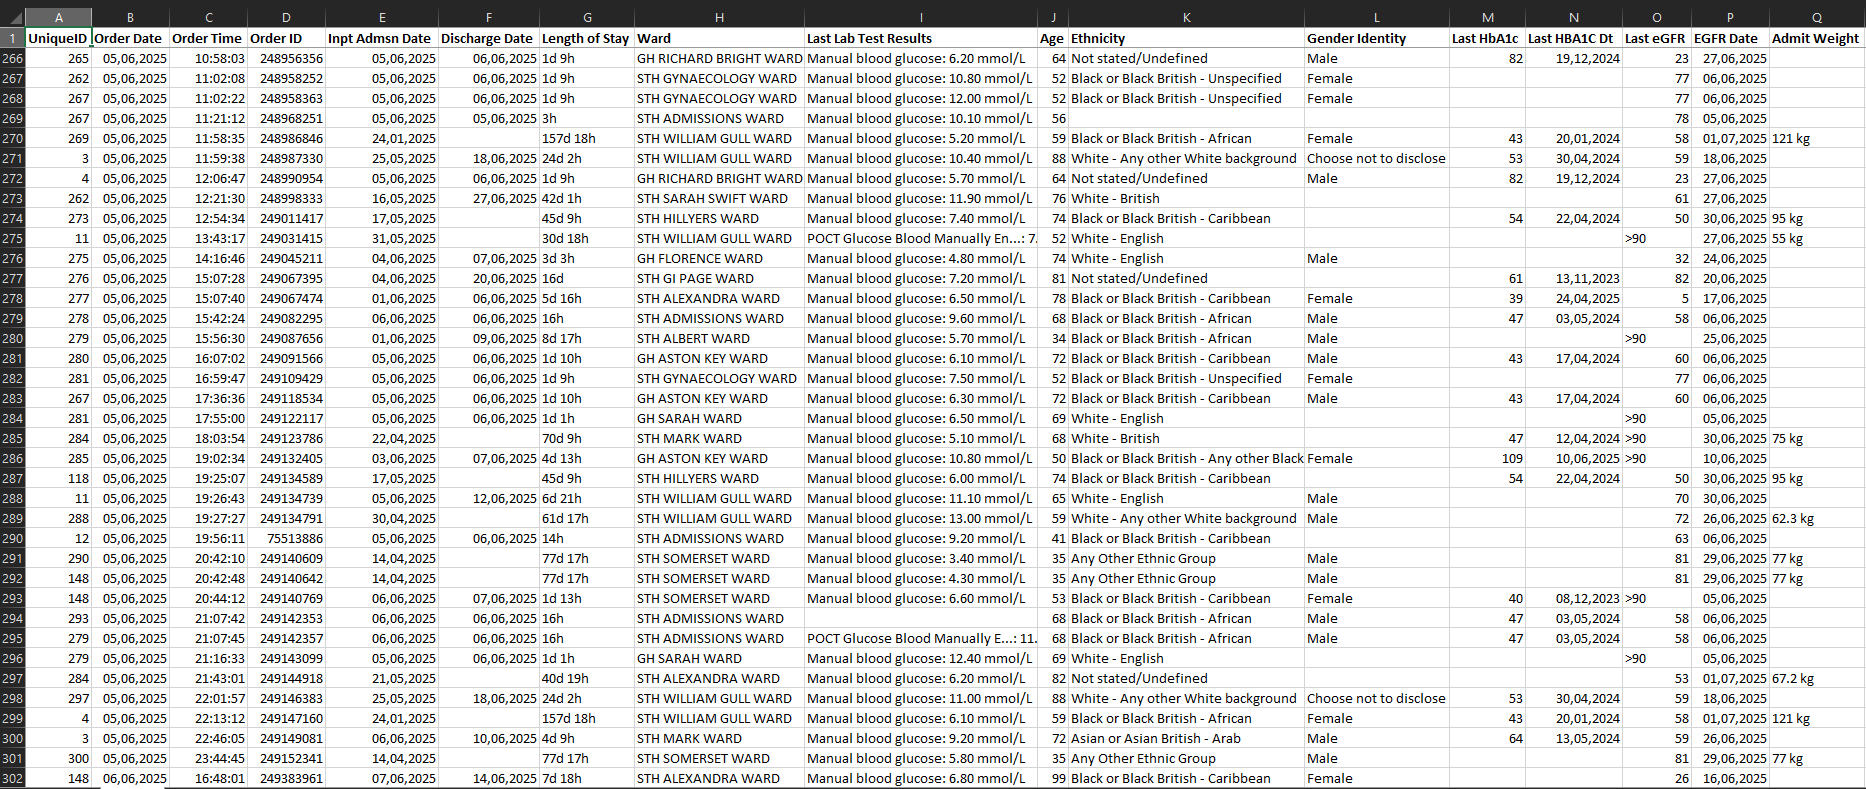
\includegraphics[width=9in, angle=90]{figures/dataset_screenshot_xl.png}
		\caption{Raw dataset}
		\label{fig:rawDataset}
	\end{figure}

	\begin{figure}[H]
		\centering
		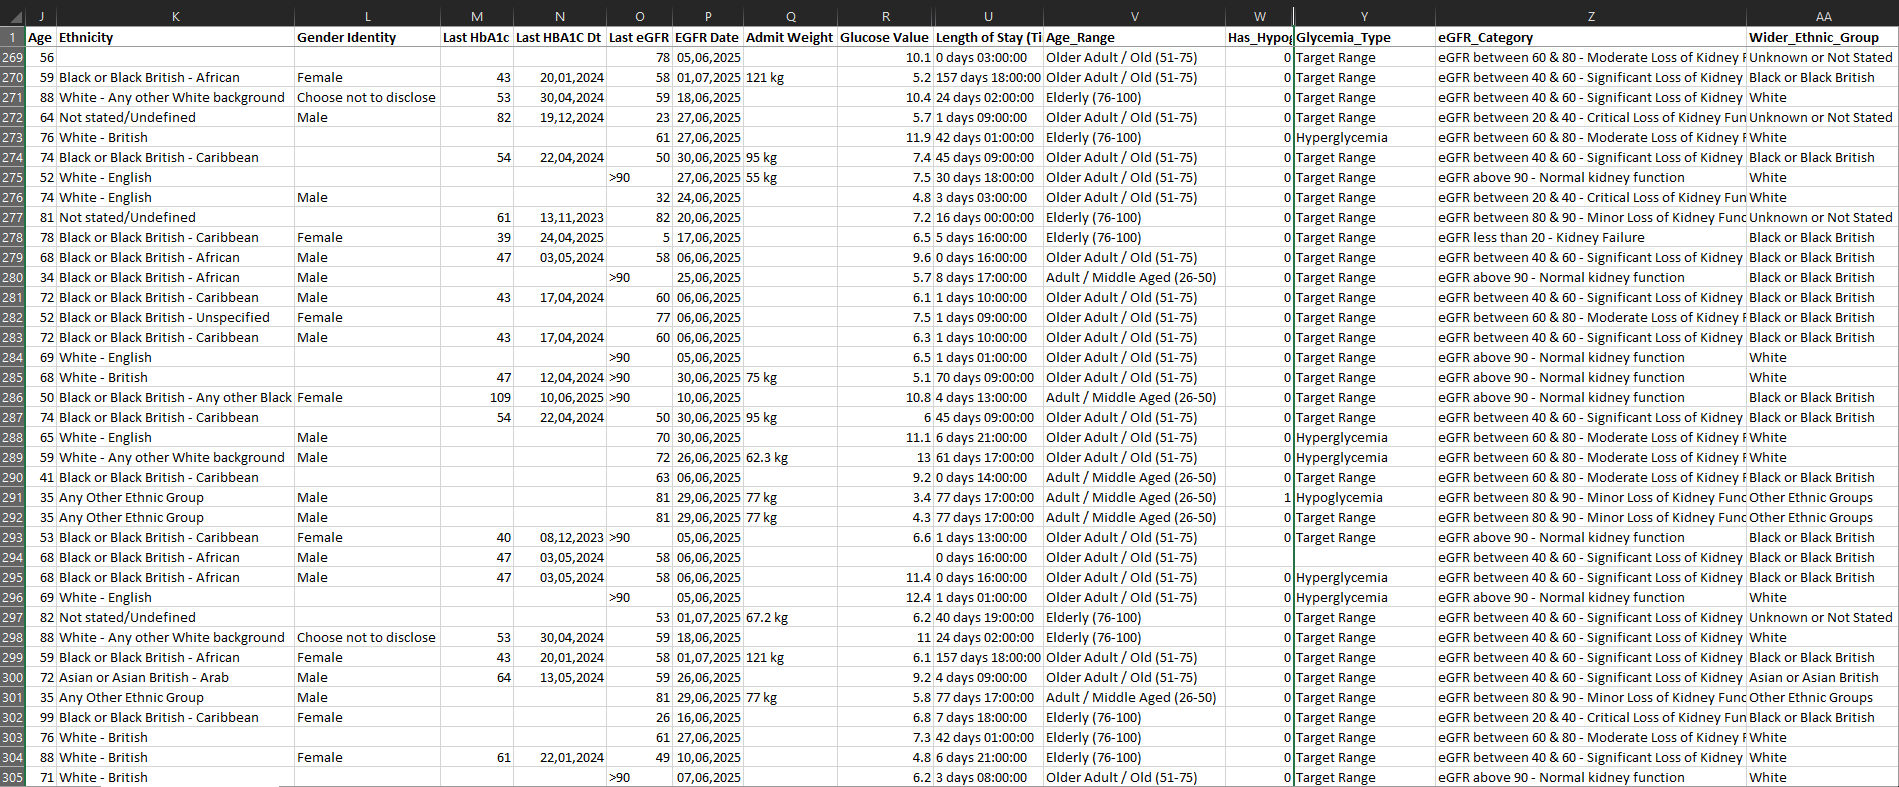
\includegraphics[width=9.5in, angle=90]{figures/cleaned_dataset_screenshot_xl.png}
		\caption{Dataset with cleaned features}
		\label{fig:cleanedDataset}
	\end{figure}

%  ===================================== TEMPLATE LEFTOVERS for ref ==========================================

% \red{The content of ``Appendix'' is in ``{\textbackslash}contents{\textbackslash}app\_1.tex''}

% \section{Appendix}
% 	Supplementary materials (such as source code, user menu, etc) could be included. Each appendix must be labelled (for example, Appendix A, Appendix A.1, Appendix A.2,  Appendix B, Appendix B.1, etc.) and with heading.  All Appendices must be referred in the text.  

% \subsection{Points to Note}
% Please note the following points when you write your report:
% \begin{itemize}
% 	\item Consider the outline of the report.  It is a good idea to start with the table of contents, which gives you an overall structure of the report.
% 	\item Show understanding of the topic and demonstrate the contribution of the work. 70\% of the content of the report should be your own contributions and achievements.
% 	\item Always use your own words.
% 	\item The main report and any appendices must constitute one document.
% 	\item Pages must be numbered consecutively.
% 	\item Captions must be provided for all figures and tables.
% 	\item Equations (or important equations), figures and tables must be numbered.
% 	\item All figures and tables must be referred to in the text.
% 	\item Units of all variables must be provided.
% 	\item Numerical values (floating-point number) should be in 4 decimal places.
% 	\item Contractions should not be used.
% 	\item Check the punctuation of sentences.  In particular, those sentences with equation.  For example, if an equation is at the end of a sentence, a full stop should be used.
% 	\item All variables must be defined.
% 	\item Font face of variables throughout the report (in the text, equation, figures and table) must be consistent.
% 	\item Use proper headings for chapters, sections, subsections.
% 	\item Chapters, sections, subsections should be numbered and with the same numbering system throughout the report.
% It is suggested that vector and matrix variables should be in bold, scalar variables should be in italic.
% 	\item References must be used for materials used in the report that are not yours.
% 	\item A standard reference format must be adopted and be consistently applied through the report.  General guidelines for reference format can be found on KEATS.
% 	\item Always backup your files.  
% \end{itemize}

% \section{Review of stochastic calculus}
% \subsection{Riemann integration}
% \subsection{The It\^o integral}



%%%%%%%%%%%%%%%%%%%%%%%%%%%%%%%%%%%%%%%%%%%%%%%%%%%%
%%%%%%%%%%%%%%%%%%%%%%%%%%%%%%%%%%%%%%%%%%%%%%%%%%%%
%%%%%%%%%%%%%%%%%%%%%%%%%%%%%%%%%%%%%%%%%%%%%%%%%%%%
%%%%%%%%%%%%%%%%%%%%%%%%%%%%%%%%%%%%%%%%%%%%%%%%%%%%


\end{document}
